\documentclass[11pt, a4paper]{article}

\usepackage[hyphens]{url}
\usepackage[pdfborder={0 0 0}]{hyperref}
\usepackage{graphicx}
\usepackage{grffile}
\graphicspath{{./pics/}{./pics-autogen/}}
\usepackage{amsmath}
\usepackage{amssymb}
\usepackage{booktabs}
\usepackage{color}
\usepackage{multirow}
\usepackage{lscape}
\usepackage[nottoc,numbib]{tocbibind}
\usepackage{charter}

\usepackage[dvipdfm, left=2.7cm, right=2.7cm, top=2.7cm, bottom=2.7cm]{geometry}


\begin{document}
\makeatletter
\renewcommand{\thefigure}{S\@arabic\c@figure}
\renewcommand{\thetable}{S\@arabic\c@table}
\makeatother
\thispagestyle{empty}
{\noindent\bf Supplementary Material of: \vspace{2em}}

{\noindent\bf ARIBA: Rapid antimicrobial resistance genotyping directly from sequencing reads\vspace{2em}}


\noindent Martin Hunt$^{1}$,
Alison E. Mather$^{1,2}$,
Leonor S\'{a}nchez-Bus\'{o}$^{1}$,
Andrew J. Page$^{1}$,
Julian Parkhill$^{1}$,
Jacqueline A. Keane$^{1}$,
Simon R. Harris$^{1}$\vspace{2em}

\noindent$^{1}$Wellcome Trust Sanger Institute, Wellcome Trust Genome Campus, Cambridge, CB10 1SA, UK


\noindent$^{2}$Department of Veterinary Medicine, University of Cambridge, Madingley Road, Cambridge, UK, CB3 0ES


\newpage
\setcounter{tocdepth}{1}
\tableofcontents
\newpage


\section{Analysis reproducibility}
Accession numbers for the raw reads are listed in
Supplementary Tables S1, S3, and S6.
All other files and scripts used for this publication
are included in the GitHub repository
\url{https://github.com/martinghunt/ariba-publication}.
This includes the reference files used as input to ARIBA,
KmerResistance, and SRST2, and how to generate them. It also
includes the output files from each tool (except for the BAM
and pileup files made by SRST2, in order to reduce space), and scripts
used to generate figures 2--5, supplementary figures
\ref{figure: e faecium read depth per gene},
\ref{figure: e faecium read depth per gene lenient},
\ref{figure: s sonnei called depth},
\ref{figure: s sonnei upset lenient},
\ref{figure: n gono AZMknowngroups_nocombos}--\ref{figure: run time and memory},
tables, and this
PDF file. We note that Figure 4 was automatically
generated by ARIBA, then the lower left labels
were tidied manually for publication. Further, a Docker
file is included so that the analysis can be easily reproduced.
Each script referred to below in this text can be found
in the \texttt{Scripts/} directory of the GitHub repository.


\section{ARIBA pipeline}
The first stage of the ARIBA pipeline is to map all read pairs to all reference
sequences, in order to produce a set of reads for each cluster of reference
sequences. Reads that map with their entire length, or overhang the end of a
reference sequence, are counted as mapped providing the match is ``good enough'',
using the following criteria. Minimap mapping coordinates are approximate
because each read is placed but is not aligned. Therefore some tolerance is allowed
at the end of each reported mapping. We allow $1.1k$ unaligned nucleotides at each
end of a read, where $k$ is the $k$-mer length used by minimap (by default
$k=15$).

\begin{figure}[h]
\begin{picture}(200,200)
\put(-20,0){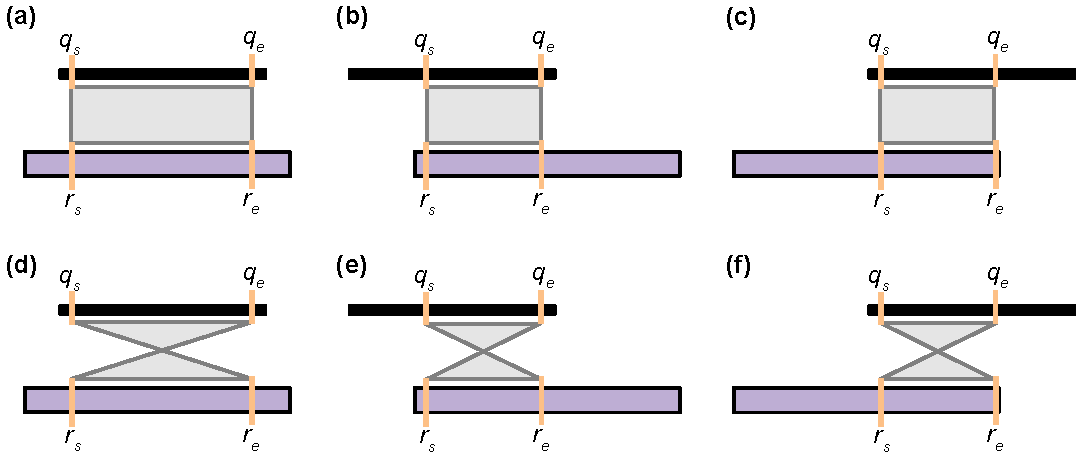
\includegraphics[width=16cm]{ariba_read_map_critera.pdf}}
\end{picture}
\caption{Visualisation of criteria used to determine whether or not a read was considered to
be mapped by minimap. See text for details.}
\label{figure: ariba read map criteria}
\end{figure}


Let $q_\ell$ and $r_\ell$ be the length of the read and reference sequences
respectively, let $\varepsilon = 1.1k$, and assume that
$q_s < q_e$ and $r_s < r_e$, where we use the labels in Supplementary Figure
\ref{figure: ariba read map criteria}.  The first requirement is that enough
of the read matches, specifically that
$$
    q_e  - q_s \geqslant \min(50, q_\ell / 2).
$$
If the read is mapped in the same orientation as the reference
(cases (a),(b),(c) in Supplementary Figure \ref{figure: ariba read map criteria}),
then we require
$$
    q_s < \varepsilon \quad \textrm{ or } \quad r_s < \varepsilon
$$
and
$$
    q_\ell - q_e < \varepsilon \quad \textrm{ or } \quad r_\ell - r_e < \varepsilon
$$
to count the read as mapped. On the other hand,
if the read is mapped onto the reverse strand of the reference
(cases (d),(e),(f) in Supplementary Figure \ref{figure: ariba read map criteria}),
then we require
$$
    q_s < \varepsilon \quad \textrm{ or } \quad r_\ell - r_e < \varepsilon
$$
and
$$
    q_\ell - q_e < \varepsilon \quad \textrm{ or } \quad r_s < \varepsilon
$$
to count the read as mapped.


If either read of a pair is counted mapped to a given reference sequence,
then that read pair is allocated to the cluster to which that reference
sequence belongs. Since for each read all mappings reported by minimap are
considered, a read pair can be allocated to more than one cluster.

Each cluster is handled using the methods described in the main text, and
outlined in Supplementary Figure \ref{figure: ariba cluster methods flowchart}.
A variety of situations can arise for each sample. The possibilities are encoded
in a bitwise flag, where each possibility is set to `true' or `false',
with the following meanings.

\begin{figure}[t]
\begin{picture}(200,490)
\put(-20,0){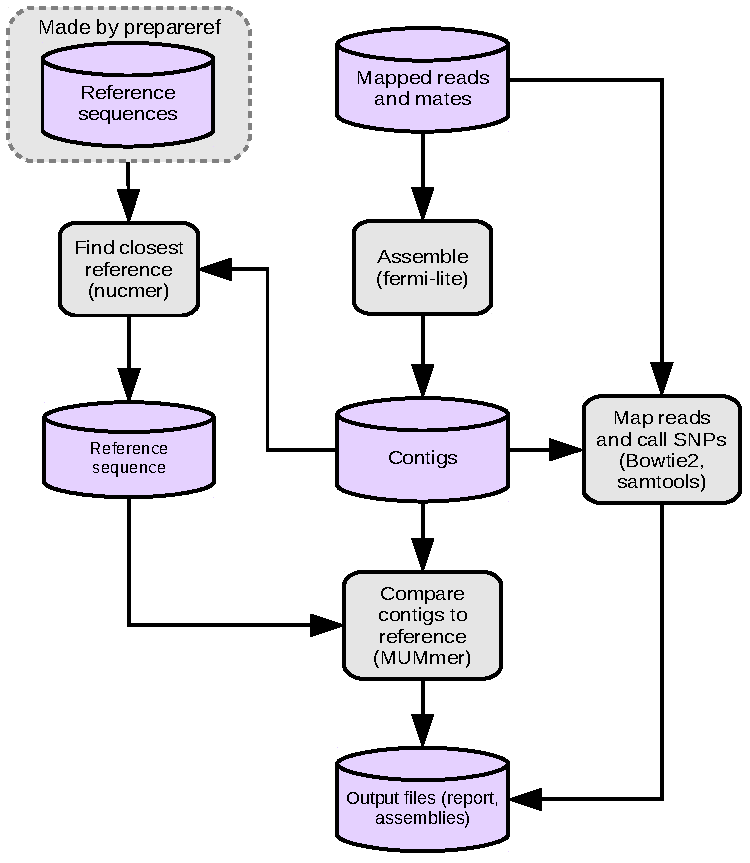
\includegraphics[height=18cm]{ariba_cluster_methods_flowchart.pdf}}
\end{picture}
\caption{Cluster processing methods (performed on each cluster during \texttt{ariba run})}
\label{figure: ariba cluster methods flowchart}
\end{figure}

\begin{itemize}
  \item \textbf{assembled:} the assembly is compared to the reference sequence using nucmer.
    If at least 95\% of the reference sequence has nucmer matches to the
    assembly, then \texttt{assembled} is true.
    The 95\% is a default value that can
    be changed with the command line option \texttt{--assembled\_threshold}.
    Note that this says nothing about how many contigs represent the gene
    (see the next option\newline \texttt{assembled\_into\_one\_contig}).

  \item \textbf{assembled\_into\_one\_contig:} this is set to true if
    \texttt{assembled} is true, and also there is a single contig with a nucmer
    match that covers at least 95\% of the reference sequence. Note that there
    could still be other contigs that match the reference (see
    \texttt{region\_assembled\_twice}).

  \item \textbf{region\_assembled\_twice:} this is set to true if more than 3\%
    of the reference sequence has more than one match to the assembly. The 3\%
    cutoff can be changed with the command line
    option \texttt{--unique\_threshold}.

  \item \textbf{complete\_gene:} if there is a match to the full length of the
    reference sequence, or if the match is not quite complete, then ARIBA
    will try to extend it to the nearest start and stop codons. If this is
    successful, and the only stop codon is at the end of the inferred gene
    sequence, then \texttt{complete\_gene} is set to true.
    This will never be set if the reference is a non-coding sequence.

  \item \textbf{unique\_contig:} this is set to true if there is exactly one
    contig in the assembly that has nucmer matches to the reference
    sequence.

  \item \textbf{scaffold\_graph\_bad:} the reads are mapped back to the
    assembly and links between the contigs from read pair information is used
    to construct a scaffolding graph. If there is any ambiguity in this
    graph, for example the end of contig A could join to the start of contig
    B or contig C, then \texttt{scaffold\_graph\_bad} is set to true.

  \item \textbf{assembly\_fail:} this is set when the assembler produces no output.
    The most likely cause is a few reads spuriously mapped to the reference
    sequence, whose depth is too low to assemble.

  \item \textbf{variants\_suggest\_collapsed\_repeat:} after mapping the reads
    back to the assembly, variants are called using samtools. If samtools
    calls any variants in any position that matches to the reference gene,
    then this is set to true. It suggests that the assembly has collapsed
    more than one sequence down into one sequence, hence the reads suggesting
    variants. Alternatively, this could be caused by a mixed input sample.

  \item \textbf{hit\_both\_strands:} this means there is a contig that has two
    (or more) matches to the reference, but the matches are in opposite
    orientations.

  \item \textbf{has\_variant:} this is set to true if there is any variant
    between the assembly and the reference. For a noncoding sequence, this
    means any nucleotide change. For a gene, this means any non-synonymous
    change. Except that a known variant is only counted when the assembly has
    the variant type, as opposed to the wild type (bear in mind that the
    reference could have the wild type or the variant type).

  \item \textbf{ref\_seq\_choose\_fail:} this is set to true if something went
    wrong when trying to find the closest reference sequence within a cluster.
\end{itemize}
ARIBA includes a utility to explain the meaning of a flag. For example,
running
\begin{verbatim}
  ariba flag 27
\end{verbatim}
results in the following output
\begin{verbatim}
  Meaning of flag 27
  [X] assembled
  [X] assembled_into_one_contig
  [ ] region_assembled_twice
  [X] complete_gene
  [X] unique_contig
  [ ] scaffold_graph_bad
  [ ] assembly_fail
  [ ] variants_suggest_collapsed_repeat
  [ ] hit_both_strands
  [ ] has_variant
  [ ] ref_seq_choose_fail
\end{verbatim}
where an \verb+X+ means that part of the flag is true. In this case, the
assembly consisted of one unique contig that included the complete gene
sequence.

Runs across multiple samples can be summarised using the \texttt{summary}
function of ARIBA, as outlined in Supplementary Figure
\ref{figure: ariba methods multiple samples}.
A key column of the output from summary is the `assembled' column,
which reports, for each sample and each gene, the status of the ARIBA
assembly. The method used to calculate this column is shown in
Supplementary Figure \ref{figure: ariba summary assembled flowchart}.


\begin{figure}[t]
\begin{picture}(200,490)
\put(-30,0){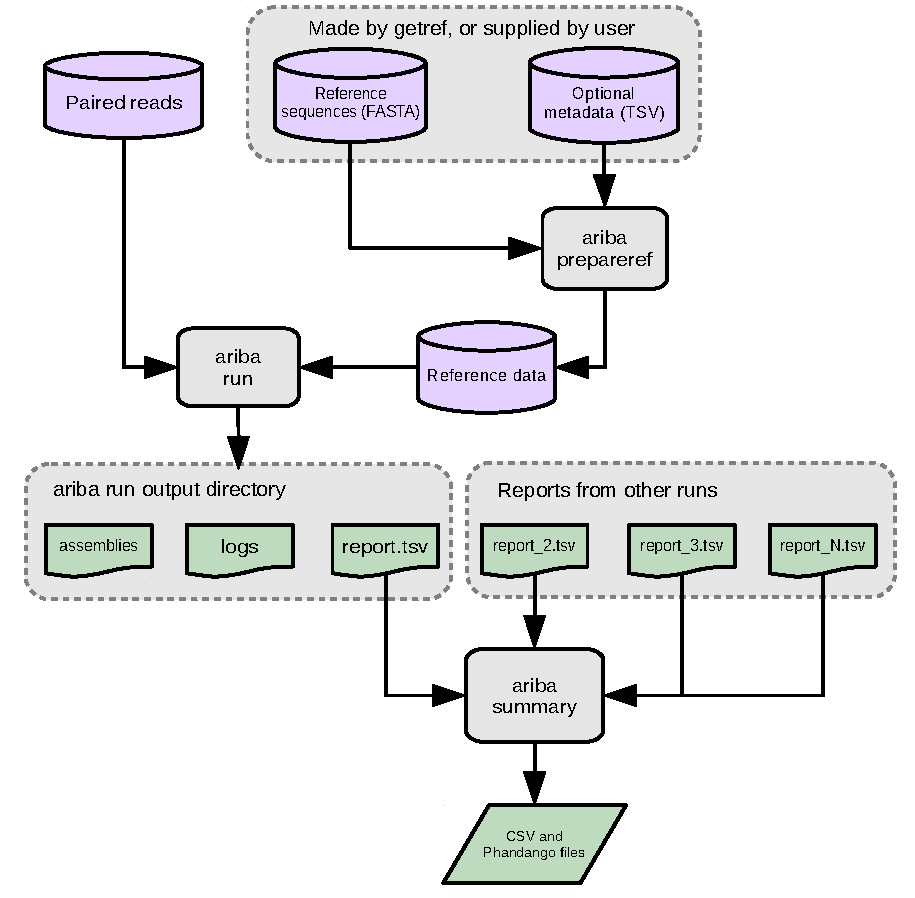
\includegraphics[width=18cm]{ariba_methods_multiple_samples.pdf}}
\end{picture}
\caption{Overview of ARIBA methods, when run on multiple samples}
\label{figure: ariba methods multiple samples}
\end{figure}

\begin{figure}[t]
\begin{picture}(200,600)
\put(10,0){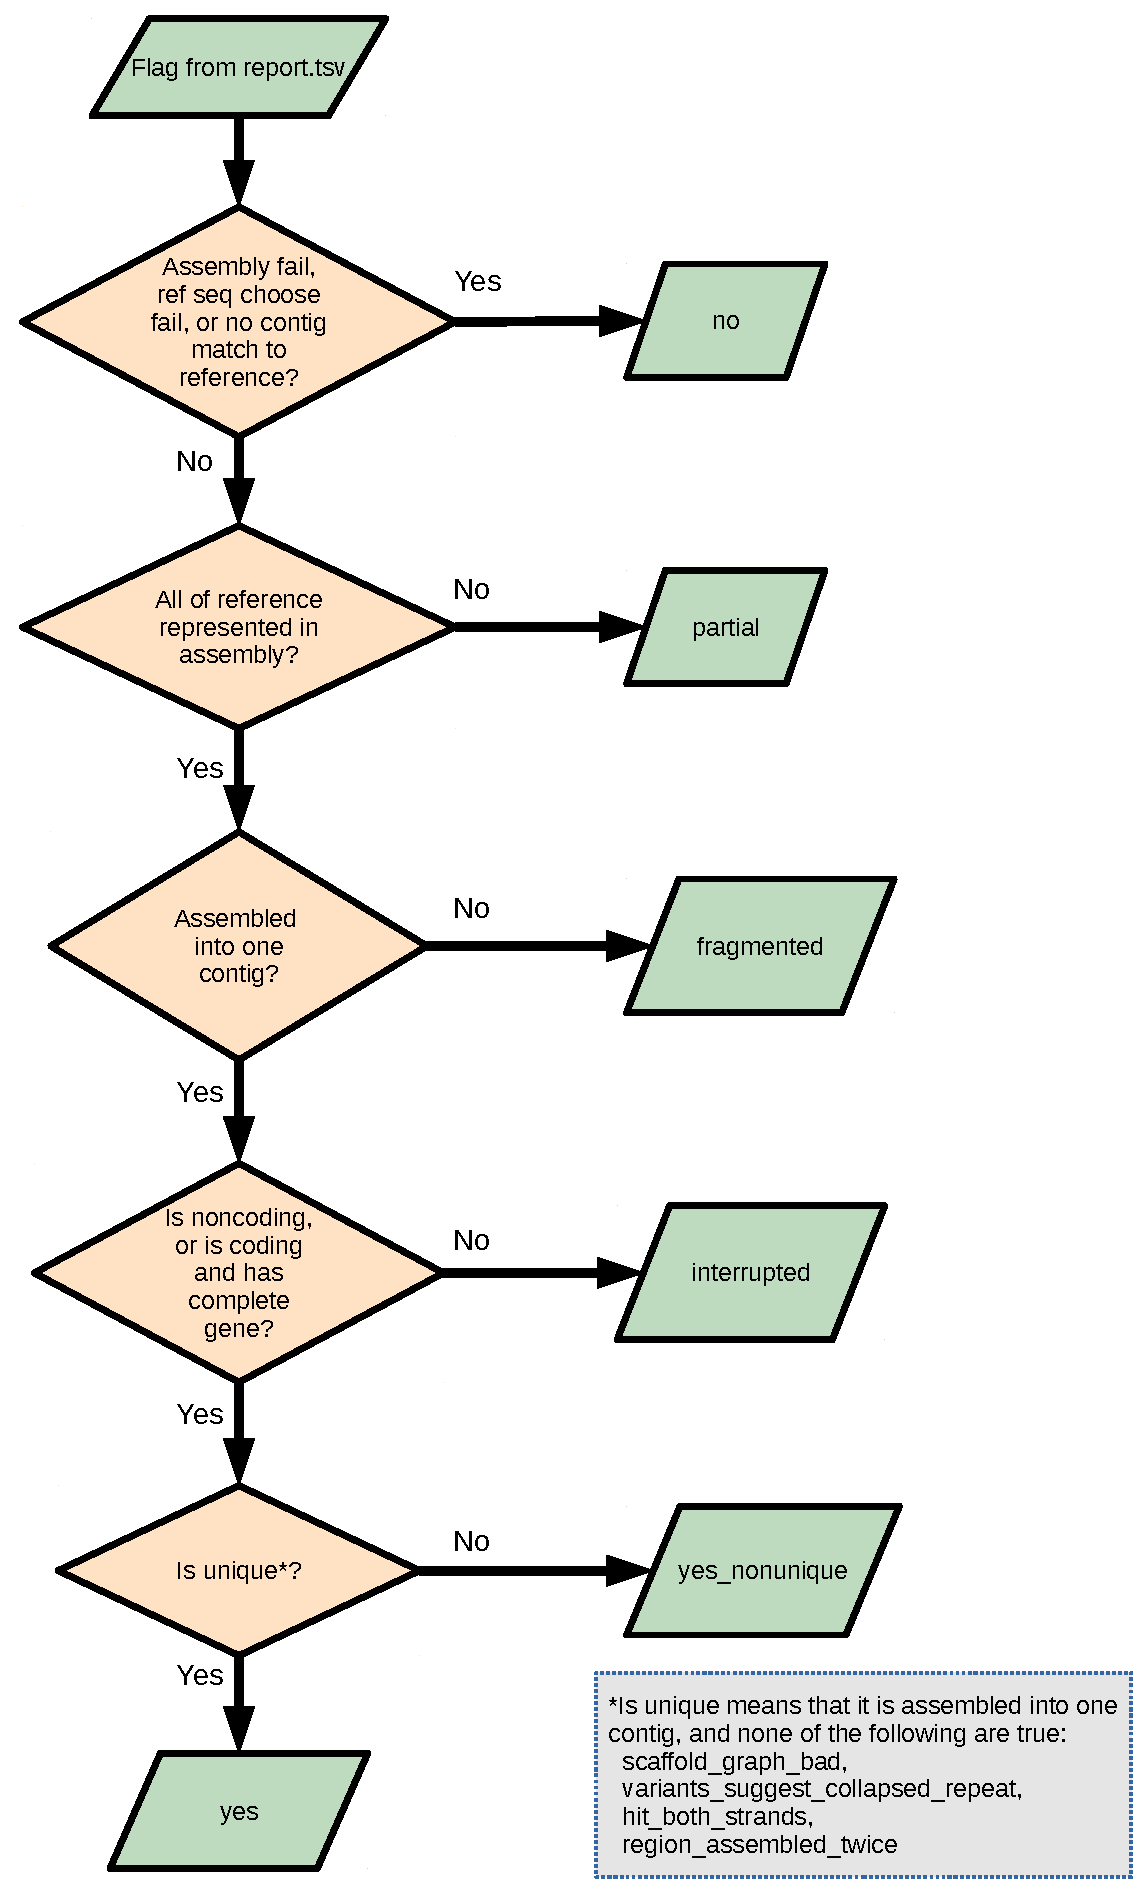
\includegraphics[width=14cm]{ariba_summary_assembled_flowchart.pdf}}
\end{picture}
\caption{Method used for calculating the `assembled' column output by \texttt{ariba summary}}
\label{figure: ariba summary assembled flowchart}
\end{figure}


\clearpage

\section{\textit{E. faecium}}
The SRST2 version of the ARG-ANNOT sequences were downloaded and formatted
for ARIBA with the following command.
\begin{verbatim}
  ariba getref srst2_argannot ariba_db.download
\end{verbatim}
The vanS-B gene, called ``47\_\_VanS-B\_Gly\_\_VanS-B\_\_1672
no;yes;VanS-B;Gly;AY655721;\newline731-2073;1343'' by SRST2, originally from
ARG-ANNOT, was missing its final nucleotide A. This was confirmed by
comparing with the GenBank record AY655721. It would cause ARIBA to exclude
this sequence because the translation into amino acids results in a sequence
that does not end with a stop codon. Therefore an “A” was added to the end of
the sequence (called ``VanS-B\_Gly.47\_\_VanS-B\_Gly\_\_VanS-B\_\_1672'') in the FASTA
file \texttt{ariba\_db.download.fa}. The data were then prepared for running the ARIBA
pipeline with the command
\begin{verbatim}
  ariba prepareref -f ariba_db.download.fa \
  -m ariba_db.download.tsv ariba_db
\end{verbatim}
and the ARIBA pipeline was run on each sample with
\begin{verbatim}
  ariba run ariba_db reads_1.fq.gz reads_2.fq.gz ariba.out
\end{verbatim}
For KmerResistance, we used the original file \texttt{ARGannot.r1.fasta}
from the
SRST2 github repository. The template database was made by running
\begin{verbatim}
  maketemplatedb.py -i ARGannot.r1.fasta -o ARGannot.r1.fasta.kres_db
\end{verbatim}
and KmerResistance was run on each sample with the command
\begin{verbatim}
  zcat reads_1.fq.gz reads_2.fz.gz | KmerResistance.py \
  -t_db ARGannot.r1.fasta.kres_db -o out1 -o2 out2 -w \
  -s_db kmerresistance/database/complete_genomes.ATGAC
\end{verbatim}
where \texttt{complete\_genomes.ATGAC} is the prefix of files that are included with KmerResistance.
SRST2 was run using the defaults options using the same reference file as
KmerResistance. The command run on each sample was:
\begin{verbatim}
  srst2 --input_pe reads_1.fq.gz reads_2.fq.gz --output out \
  --log --gene_db ARGannot.r1.fasta
\end{verbatim}


\subsection{MLST calling}
For MLST calling, the ARIBA reference data was downloaded from
PubMLST and formatted for use with ARIBA using the command
\begin{verbatim}
  ariba pubmlstget 'Enterococcus faecium' ariba_db.mlst
\end{verbatim}
and ARIBA was run on each sample with
\begin{verbatim}
  ariba run ariba_db.mlst/ref_db reads_1.fq.gz reads_2.fq.gz ariba.out
\end{verbatim}
The reference data was downloaded for SRST2 using the command
\begin{verbatim}
  getmlst.py --species "Enterococcus faecium"
\end{verbatim}
where \verb+getmlst.py+ is the script included with SRST2, and
then SRST2 was run on each sample with the command
\begin{verbatim}
  srst2 --input_pe reads_1.fq.gz reads_2.fq.gz --output out \
  --log --mlst_db Enterococcus_faecium.fasta \
  --mlst_definitions srst2_pubmlst/efaecium.txt \
  --mlst_delimiter '_'
\end{verbatim}


\subsection{Investigation of 7 genes in VanB operon}


Only the VanB cluster had more than one gene. All tools gave the same
reference sequence (where the gene was present), except for SRR980582, where
ARIBA and SRST2 chose \texttt{VanB\_1058} and KmerResistance
chose \texttt{VanB\_1060}.


All other differences were in the presence/absence of genes. Several of the
differences were in samples genotyped to be VSE (see Supplemetary Table S1),
where the differences appear to be due to marginal calls from low level
contamination. The remaining differences, discussed below, were all in VRE
samples.

All tools agreed for \textit{vanB}, \textit{vanH}, \textit{vanR},
\textit{vanS}, and \textit{vanX}, the differences were
all in \textit{vanW} and \textit{vanY}.


\paragraph{\textit{vanW}.}
Samples SRR980557, SRR980566, SRR980567, SRR980576, SRR980580, SRR980581,
and SRR9805803
were called by ARIBA as having nonsense mutations, and
SRR980574 with a frameshift. SRST2 called all these samples as ``VanW-B\_487*?'',
except for  SRR980557 which was called as ``VanW-B\_487*'' suggesting that it is
present in the sample. KmerResistance reported all these samples as having
the \textit{vanW} gene. Further, ARIBA reported that
the seven nonsense mutations were identical, changing the amino acid W
to a stop codon at nucleotide position 571 in the reference gene. This
was confirmed by running the
following command on each BAM file output by SRST2:
\begin{verbatim}
  samtools mpileup -L 100000 -t INFO/AD -A -f ARGannot.r1.fasta \
   -u -v -r 239__VanW-B_Gly__VanW-B__487:571-573 in.bam
\end{verbatim}
where it was clear from the output that the codon TGG in the reference
gene was changed to TGA in each sample. For example, the following lines
are output from sample SRR980583
\begin{verbatim}
239__VanW-B_Gly__VanW-B__487 571 . T <*>   0 . DP=612;AD=591,0;
239__VanW-B_Gly__VanW-B__487 572 . G <*>   0 . DP=611;AD=585,0;
239__VanW-B_Gly__VanW-B__487 573 . G A,<*> 0 . DP=589;AD=0,564,0;
\end{verbatim}
where each line has been truncated to fit on the page, with just the relevant
information shown.




\paragraph{\textit{vanY} in sample SRR980559.}
This was called by ARIBA and SRST2, but not by KmerResistance. ARIBA reported 17
nonsynonymous amino acid changes, and SRST2 reported ``44snp1indel''. Given
that ARIBA reported 94.42\% identity between its assembly and the reference
gene, we assume that the sample was too distant to be identified by
KmerResistance.


\paragraph{\textit{vanY} in sample SRR980565.} This was called by KmerResistance,
with 95\% coverage, but
not by ARIBA or SRST2. ARIBA produced an assembly of 670 of the 807bp gene at
100\% identity, therefore reporting the gene as not present. This was
confirmed upon viewing the BAM file produced by SRST2, as shown in
Supplementary Figure \ref{figure: e faecium SRR980565 artemis}.

\begin{figure}[t]
\begin{picture}(200,500)
\put(-50,340){\includegraphics[clip=true, trim=0 0 4.5cm 0, height=4.4cm]{e_faecium.depth_plot.VanB.pdf}}
\put(230,340){\includegraphics[clip=true, trim=0 0 4.5cm 0, height=4.4cm]{e_faecium.depth_plot.VanH.pdf}}
\put(-50,170){\includegraphics[clip=true, trim=0 0 4.5cm 0, height=4.4cm]{e_faecium.depth_plot.VanR.pdf}}
\put(230,170){\includegraphics[clip=true, trim=0 0 4.5cm 0, height=4.4cm]{e_faecium.depth_plot.VanS.pdf}}
\put(-50,0){\includegraphics[clip=true, trim=0 0 4.5cm 0, height=4.4cm]{e_faecium.depth_plot.VanX.pdf}}
\put(230,0){\includegraphics[height=4cm, clip=true, trim=16cm 2cm 0 2cm]{e_faecium.depth_plot.VanX.pdf}}
\put(-55,470){\textbf{(a)} \textit{vanB}}
\put(225,470){\textbf{(b)} \textit{vanH}}
\put(-55,300){\textbf{(c)} \textit{vanR}}
\put(225,300){\textbf{(d)} \textit{vanS}}
\put(-55,130){\textbf{(e)} \textit{vanX}}
\end{picture}
\caption{Effect of read depth on calling genes on \textit{E. faecium} dataset.}
\label{figure: e faecium read depth per gene}
\end{figure}


\begin{figure}[t]
\begin{picture}(200,610)
\put(-50,490){\includegraphics[clip=true, trim=0 0 4.5cm 0, height=4.4cm]{e_faecium.lenient.depth_plot.VanB.pdf}}
\put(230,490){\includegraphics[clip=true, trim=0 0 4.5cm 0, height=4.4cm]{e_faecium.lenient.depth_plot.VanH.pdf}}
\put(-50,320){\includegraphics[clip=true, trim=0 0 4.5cm 0, height=4.4cm]{e_faecium.lenient.depth_plot.VanR.pdf}}
\put(230,320){\includegraphics[clip=true, trim=0 0 4.5cm 0, height=4.4cm]{e_faecium.lenient.depth_plot.VanS.pdf}}
\put(-50,150){\includegraphics[clip=true, trim=0 0 4.5cm 0, height=4.4cm]{e_faecium.lenient.depth_plot.VanX.pdf}}
\put(230,150){\includegraphics[clip=true, trim=0 0 4.5cm 0, height=4.4cm]{e_faecium.lenient.depth_plot.all.pdf}}
\put(100,10){\includegraphics[height=4cm, clip=true, trim=16cm 2cm 0 2cm]{e_faecium.lenient.depth_plot.all.pdf}}
\put(-55,620){\textbf{(a)} \textit{vanB}}
\put(225,620){\textbf{(b)} \textit{vanH}}
\put(-55,450){\textbf{(c)} \textit{vanR}}
\put(225,450){\textbf{(d)} \textit{vanS}}
\put(-55,280){\textbf{(e)} \textit{vanX}}
\put(225,280){\textbf{(f)} All genes}
\end{picture}
\caption{Effect of read depth on calling genes on \textit{E. faecium} dataset, with
more permissive criteria than those used in the main manuscript and in
Supplementary Figure \ref{figure: e faecium read depth per gene}.
Here, we additionally include calls made by SRST2 with a ``?'', and calls made by ARIBA
where the assembly is identified as partial, fragmented, or interrupted.}
\label{figure: e faecium read depth per gene lenient}
\end{figure}


\begin{figure}[t]
\begin{picture}(200,300)
\put(30,0){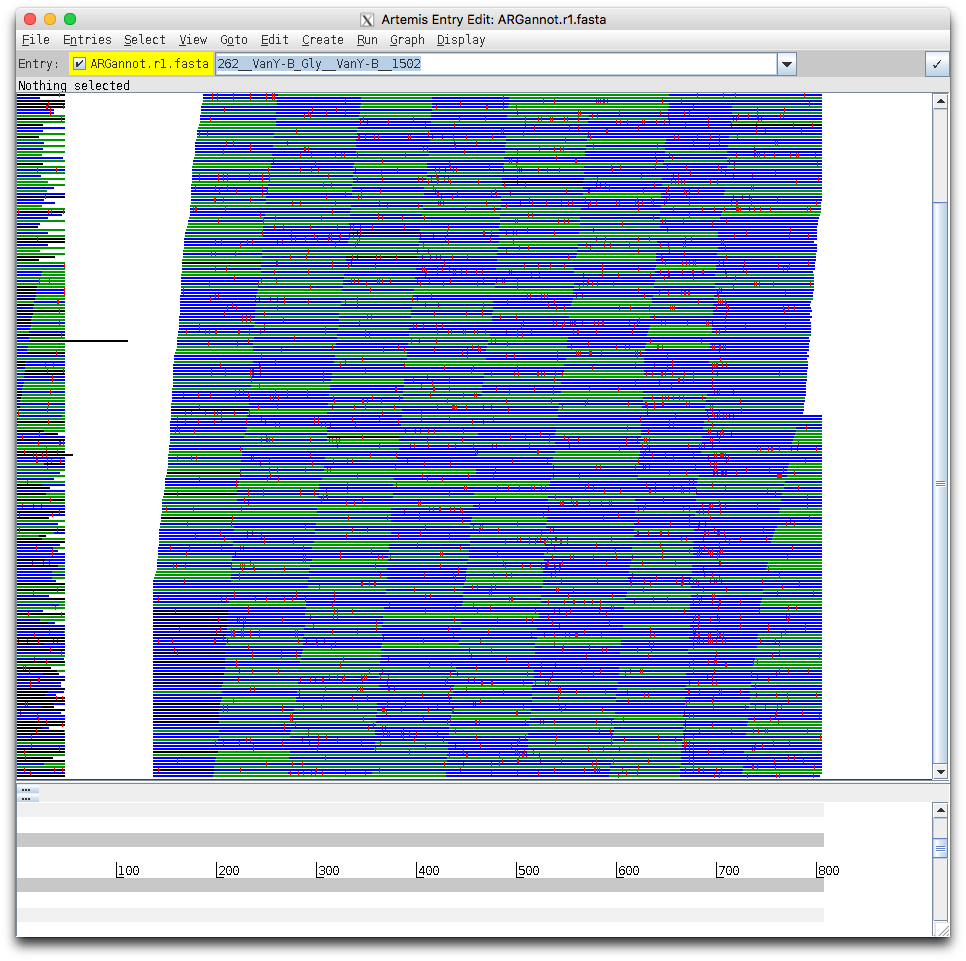
\includegraphics[width=10cm]{e_faecium.SRR980565.artemis.png}}
\end{picture}
\caption{Artemis screenshot showing reads from sample SRR980565 mapped to
the \textit{vanY} gene.}
\label{figure: e faecium SRR980565 artemis}
\end{figure}



\paragraph{\textit{vanY} in sample SRR980581.}
ARIBA called this as ``interrupted'' because of a
frameshift. SRST2 reported ``VanY-B\_1502*'', with ``1indel'', and KmerResistance
reported it as present, with 100\% coverage of the
gene.

The frameshift was verified by running the folloing command
on the BAM file made by SRST2
\begin{verbatim}
  samtools mpileup -L 100000 -t INFO/AD -A \
   -f ARGannot.r1.fasta -u -v \
   -r 262__VanY-B_Gly__VanY-B__1502 out__reads.ARGannot.r1.sorted.bam \
   | bcftools call -c -v -
\end{verbatim}
which reported this:
\begin{verbatim}
262__VanY-B_Gly__VanY-B__1502 122 . TGGGG TGGGGG 214.458 .
  INDEL;IDV=974;IMF=0.879855;DP=1107;AD=1,795;VDB=0.0048673;SGB=-0.693147;
  MQSB=1;MQ0F=0;AF1=1;AC1=2;DP4=0,1,434,361;MQ=20;FQ=-289.528;
  PV4=0.454774,1,1,0.240182   GT:PL   1/1:255,255,0
\end{verbatim}
ie a one base insertion in the reads, supported at high quality by 795 of the
796 reads mapped to that location.




\clearpage

\section{\emph{S. sonnei}}

\subsection{Reference data}
The extra reference sequences, the details of which are in
Supplementary Table S4,  were downloaded using the script
\verb+s_sonnei_get_extra_ref_seqs.py+. The CARD data was downloaded
with the command
\begin{verbatim}
   ariba getref --version 1.1.2 card card.getref
\end{verbatim}
and prepared to run with ARIBA by running
\begin{verbatim}
  ariba prepareref -f card.getref.fa -m card.getref.tsv \
   -f ref_data.sequences.fa -m ref_data.metadata.tsv ariba_db
\end{verbatim}
The reference sequences were written to a FASTA file,
\verb+srst2.fa+, compatible
for use with SRST2 by running
\begin{verbatim}
  make_srst2_fa.py ariba_db srst2.fa
\end{verbatim}
Finally, the data were prepared for use with KmerResistance using
the two commands
\begin{verbatim}
  sed 's/_/-/g' ariba_db/02.cdhit.all.fa > kres_db.input.fa

  maketemplatedb.py -i kres_db.input.fa -o kres_db
\end{verbatim}


A comparison of read depth of genes called by ARIBA and KmerResistance
shown in Supplementary Figure \ref{figure: s sonnei called depth}.

A comparison of ARIBA local assembly and reference \emph{strA} gene for sample
ERR024606 shown in Supplementary Figure \ref{figure: s sonnei ERR024606 ACT}, and for
\emph{strB} and ERR024606 in Supplementary Figure \ref{figure: s sonnei ERR028673 ACT}.



\subsection{Verify \emph{gyrA} SNPs}
The following command was used on the SRST2 BAM file for samples
ERR028676 and ERR028677 to verify the presence or absence of one of the
SNPs S83L, D87G, or D87Y:
\begin{verbatim}
samtools mpileup -L 100000 -t INFO/AD -A -f srst2.fa -uv \
 -r 569__gyrA-7__gyrA.3003294.U00096.2336792-2339420.2052__1821:$start-$end \
 in.bam
\end{verbatim}
where \verb+$start-$end+ took the values \verb+247-249+ and
\verb+259-261+. The output for sample ERR028676 was
\begin{verbatim}
569__gyrA-7__gyrA.3003294.U00096.2336792-2339420.2052__1821 247 . T <*> 0
  . DP=170;AD=168,0;
569__gyrA-7__gyrA.3003294.U00096.2336792-2339420.2052__1821 248 . C <*> 0
  . DP=170;AD=169,0;
569__gyrA-7__gyrA.3003294.U00096.2336792-2339420.2052__1821 249 . G <*> 0
  . DP=171;AD=171,0;
569__gyrA-7__gyrA.3003294.U00096.2336792-2339420.2052__1821 259 . G <*> 0
  . DP=172;AD=167,0;
569__gyrA-7__gyrA.3003294.U00096.2336792-2339420.2052__1821 260 . A <*> 0
  . DP=173;AD=173,0;
569__gyrA-7__gyrA.3003294.U00096.2336792-2339420.2052__1821 261 . C <*> 0
  . DP=173;AD=173,0;
\end{verbatim}
confirming that none of the SNPs of interest were present. The output
for sample ERR028677 was
\begin{verbatim}
569__gyrA-7__gyrA.3003294.U00096.2336792-2339420.2052__1821 247 . T <*> 0
  . DP=31;AD=31,0;
569__gyrA-7__gyrA.3003294.U00096.2336792-2339420.2052__1821 248 . C T,<*> 0
  . DP=30;AD=0,30,0;
569__gyrA-7__gyrA.3003294.U00096.2336792-2339420.2052__1821 249 . G <*> 0
  . DP=30;AD=30,0;
569__gyrA-7__gyrA.3003294.U00096.2336792-2339420.2052__1821 259 . G <*> 0
  . DP=30;AD=29,0;
569__gyrA-7__gyrA.3003294.U00096.2336792-2339420.2052__1821 260 . A <*> 0
  . DP=30;AD=29,0;
569__gyrA-7__gyrA.3003294.U00096.2336792-2339420.2052__1821 261 . C <*> 0
  . DP=31;AD=30,0;
\end{verbatim}
confirming the SNP S83L (a codon change from TCG to TTG).


\begin{figure}[h]
\begin{picture}(200,450)
\put(0,200){\includegraphics[width=17cm]{s_sonnei.called_depth.pdf}}
\put(0,0){\includegraphics[width=17cm]{s_sonnei.called_depth.0-150.pdf}}
\put(-10,380){\bf (a)}
\put(-10,180){\bf (b)}
\end{picture}
\caption{Comparison of read depth of genes called by ARIBA, KmerResistance and SRST2
on the \emph{S. sonnei} data set. (a) shows all values of reported read depths, whereas
(b) shows only the range 0--150, so that the details are visible at low depth.}
\label{figure: s sonnei called depth}
\end{figure}


\begin{figure}
\begin{picture}(200,350)
\put(-20,0){\includegraphics[width=18cm]{s_sonnei.lenient.upset.pdf}}
\end{picture}
\caption{Concordance between AMR calling methods on the \emph{S. sonnei} data.
A coloured dot indicates which methods were in agreement. The first column
illustrates where no resistance mechanisms were predicted. This is generated
using more permissive rules than in Figure 2.
Here, we additionally include calls made by SRST2 with a ``?'', and
calls made by ARIBA
where the assembly is identified as partial, fragmented, or interrupted.}
\label{figure: s sonnei upset lenient}
\end{figure}


\begin{figure}
\begin{picture}(200,350)
\put(-30,0){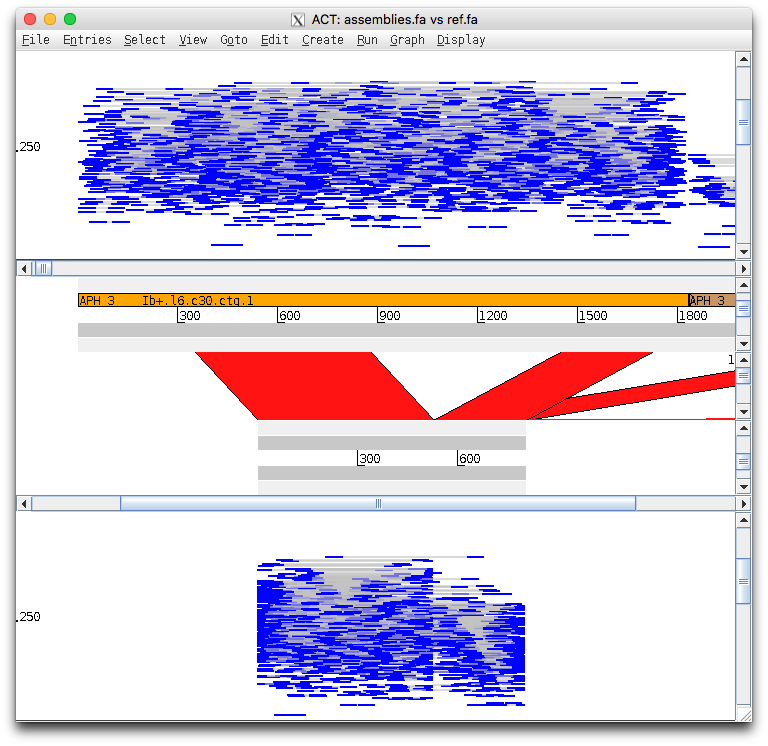
\includegraphics[width=17cm]{shigella.ERR024606.ACT.strA.png}}
\end{picture}
\caption{Sample ERR024606 \emph{strA} gene. ACT screenshot showing a comparison
between the ARIBA assembly (top) of \textit{strA}
and the reference sequence (bottom).
Nucmer matches between the sequences are shown in red. The mapped reads are
shown in ``inferred size'' view, where reads are shown in blue, with each pair
connected with a grey line. The height of each read pair is determined by the
inferred insert size from the mapping. The BAM file made by SRST2 was used
for the reference sequence, and the reads were mapped to the ARIBA contigs
using Bowtie2 with the default settings. The position of the insertion is
clear in the reads mapped to the reference sequence, whereas there is
consistent coverage across the ARIBA assembly.}
\label{figure: s sonnei ERR024606 ACT}
\end{figure}


\begin{figure}
\begin{picture}(200,350)
\put(-30,0){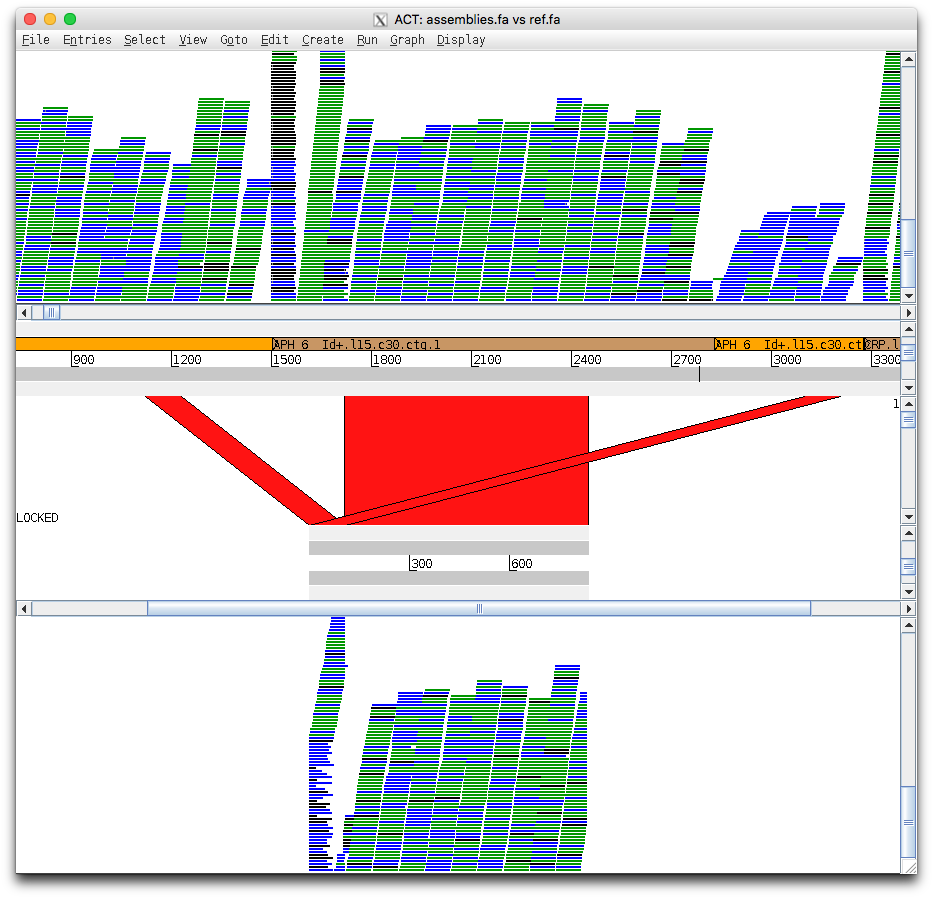
\includegraphics[width=18cm]{shigella.ERR028673.ACT.strB.png}}
\end{picture}
\caption{Sample ERR028673 \emph{strB} gene, showing a comparison of the ARIBA
assembly (top) and the reference sequence (bottom) together with the mapped
reads. Reads were mapped in the same way as explained for Supplementary
Figure \ref{figure: s sonnei ERR024606 ACT}.}
\label{figure: s sonnei ERR028673 ACT}
\end{figure}


\clearpage


\newpage
\section{\emph{N. gonorrhoeae}}
The reference data were prepared for ARIBA using the methods described in the main text.
The workflow is automated in the script
\texttt{n\_gonorrhoeae\_make\_ariba\_db.sh}, which contains all the
commands that were used.



\begin{figure}[h]
\begin{picture}(200,330)
\put(-40,0){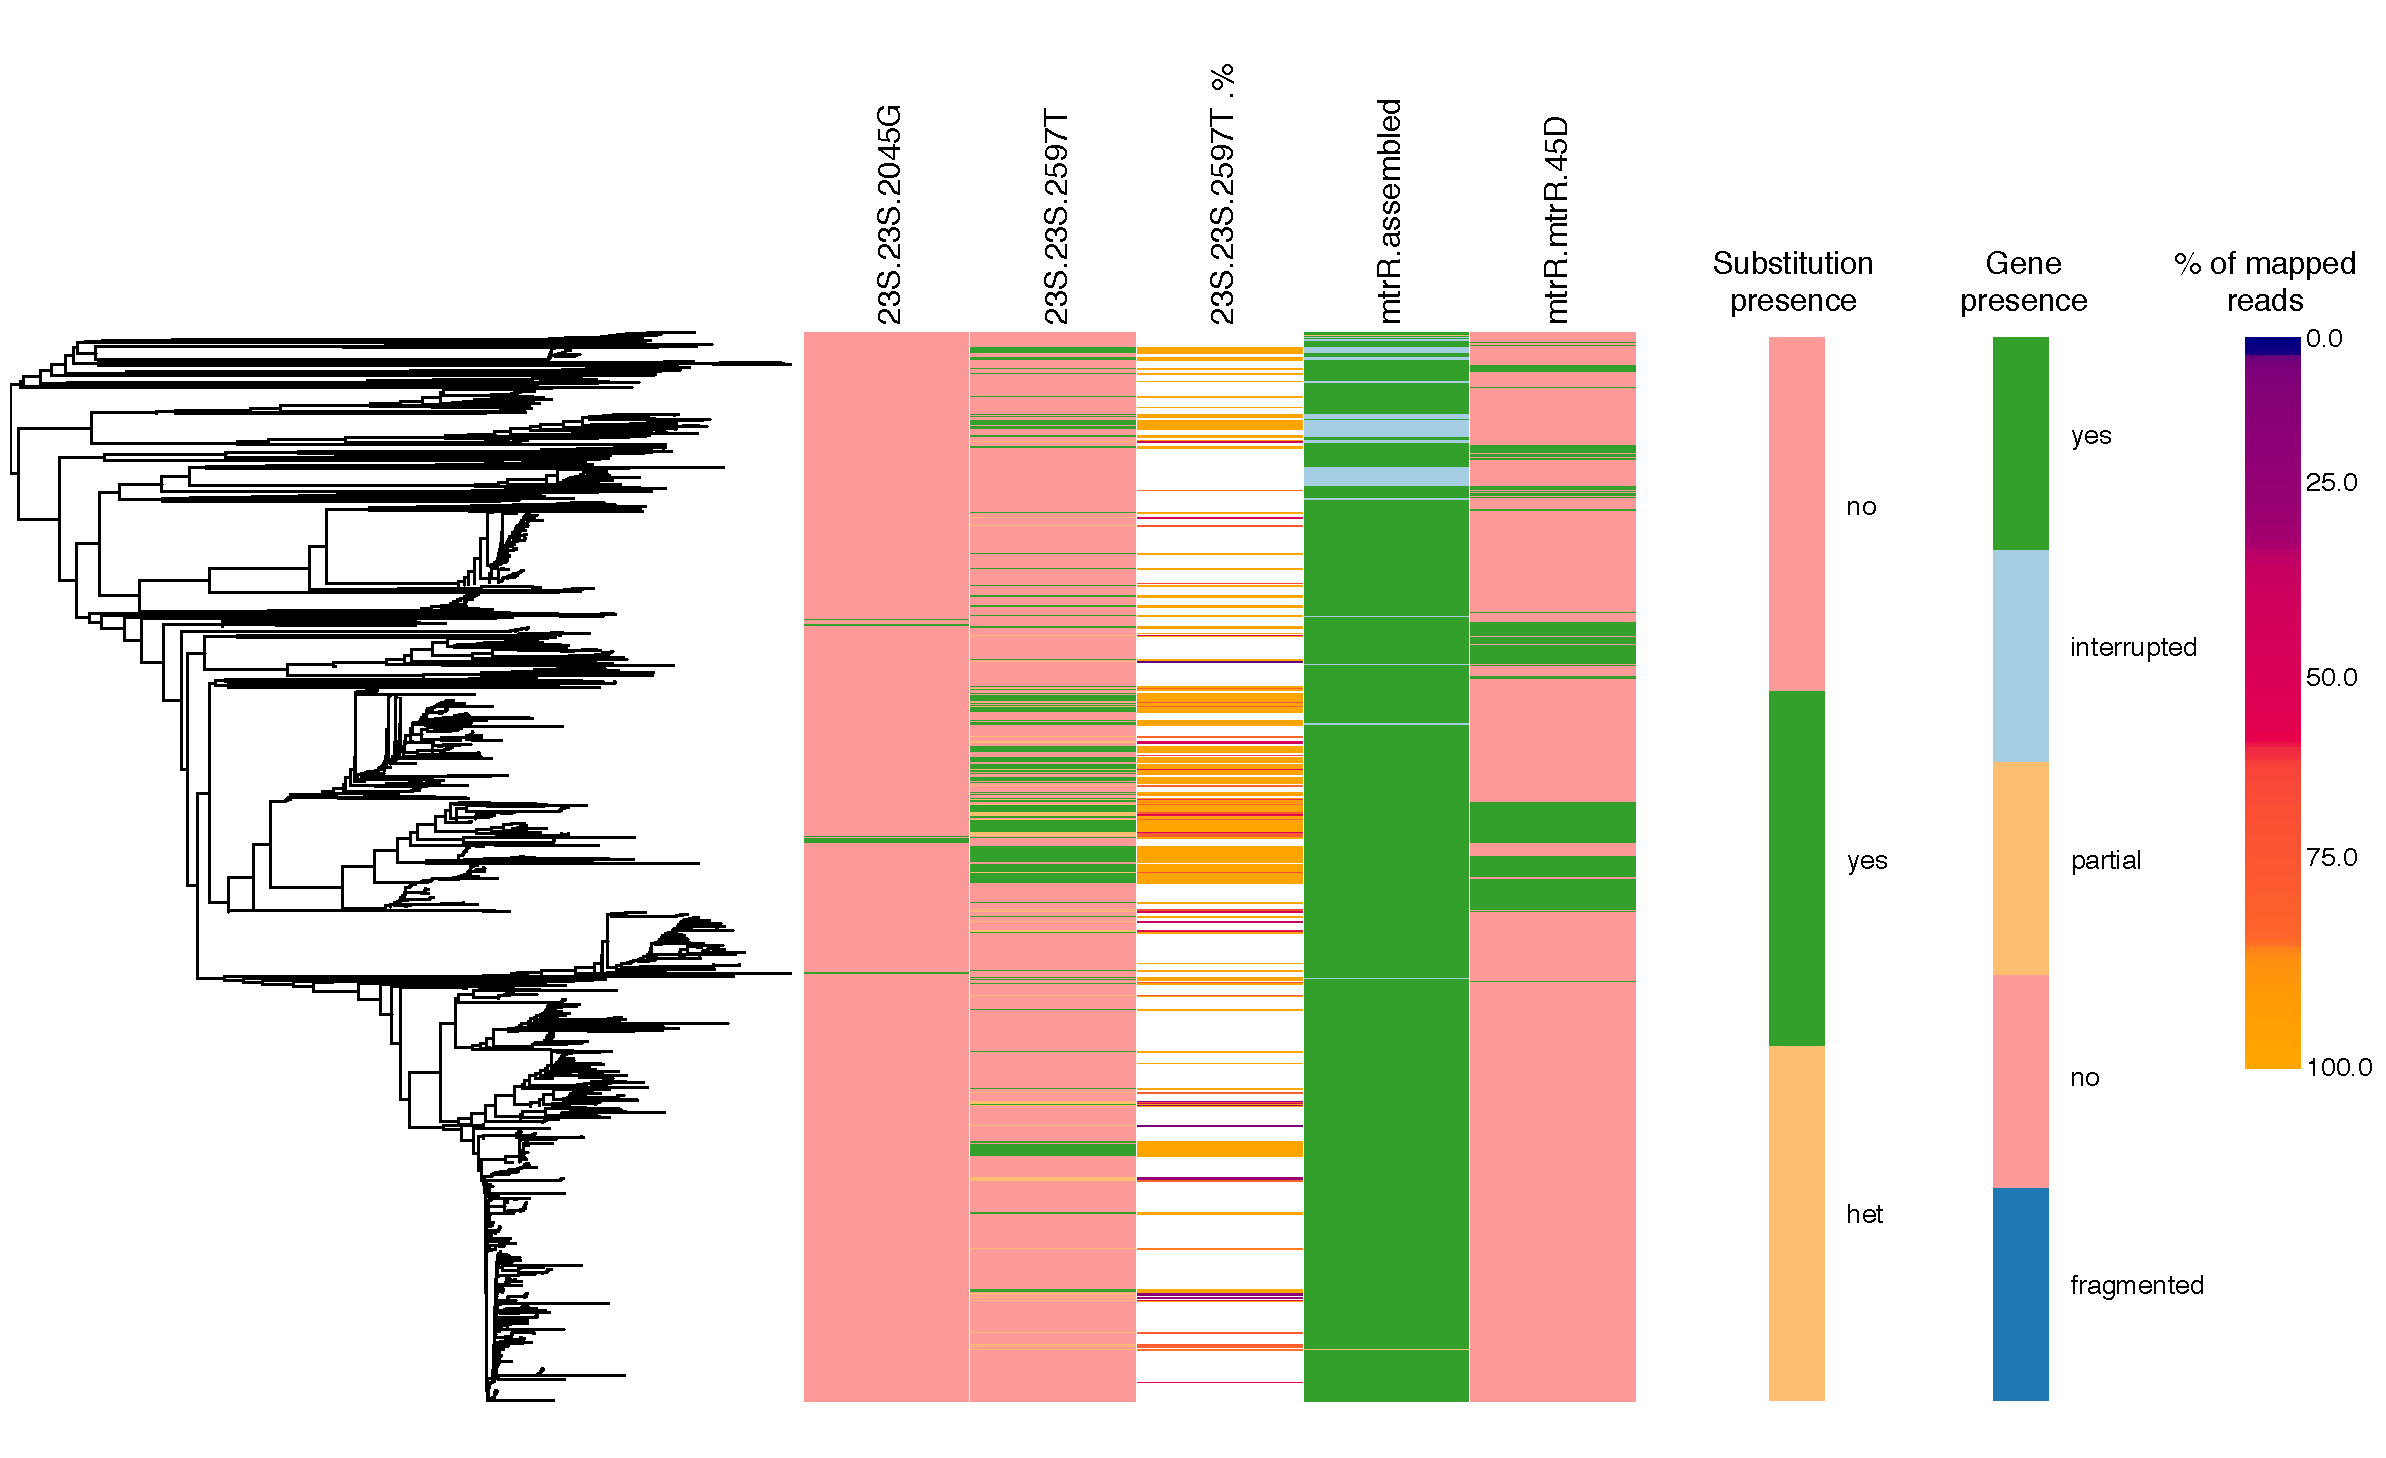
\includegraphics[width=18cm]{n_gono.phandango_plot.pdf}}
\end{picture}
\caption{Phandango visualisation of ARIBA
results for \textit{N. gonorrhoeae}
aligned against a phylogentic tree of the isolates
to illustrate that resistance determinants have emerged multiple times in the
population. Colours in columns showing the presence (yes) or absence (no) of a
particular substitution are indicated in the substitution presence key. For
the 23S C2597T substitution the percentage of mapped reads containing the
substitution are shown in the 2597T.\% column,
for which the key is labelled \%
of mapped reads. The meaning of colours in the metR.assembled column are shown
in the gene presence key, and indicate isolates for which the assembly for the
\emph{mtrR} gene is complete (yes),
interrupted, partial, fragmented or absent (no).}
\label{figure: n gono pahandango}
\end{figure}


\begin{figure}[h]
\begin{picture}(200,300)
\put(0,0){\includegraphics[width=16cm]{n_gono_AZMknowngroups_nocombos.pdf}}
\end{picture}
\caption{
Distribution of MICs (represented on a logarithmic scale) for
azithromycin for all relevant AMR determinants in our custom database. Dotted
horizontal lines mark clinical breakpoints as described in Figure
4.}
\label{figure: n gono AZMknowngroups_nocombos}
\end{figure}

\begin{figure}[h]
\begin{picture}(200,300)
\put(0,0){\includegraphics[width=16cm]{n_gono_AZMknowngroups_nohets.pdf}}
\end{picture}
\caption{
Distribution of MICs (represented on a logarithmic scale) for
azithromycin for all observed combinations of relevant AMR determinants in our
custom database excluding heterozygous hits. Dotted horizontal lines mark
clinical breakpoints as described in Figure 4.}
\label{figure: n gono AZMknowngroups_nohets}
\end{figure}



\clearpage
\newpage

\section{Run time and memory}
Box plots of the run time and memory are shown in Supplementary Figure
\ref{figure: run time and memory}  for
the \textit{E. faecium} and \textit{S. sonnei} data sets. The values used for wall
clock time and peak memory usage were those reported from using
the UNIX command \texttt{time -v}. Specifically, wall clock time is taken
from the value of ``Elapsed (wall clock) time'' and peak memory from the
value of ``Maximum resident set size''.
The raw data are given in Supplementary Table S2, and original output
from \texttt{time -v} is included in the GitHub repository.



\begin{figure}[h]
\begin{picture}(200,470)
\put(10,230){\includegraphics[width=16cm]{resources.time.pdf}}
\put(10,0){\includegraphics[width=16cm]{resources.ram.pdf}}
\put(0, 440){\bf(a)}
\put(0, 210){\bf(b)}
\end{picture}
\caption{(a) Run time and (b) memory usage on the \emph{E. faecium} and
\emph{S. sonnei} datsets.}
\label{figure: run time and memory}
\end{figure}


\end{document}
